\documentclass{homework}
\newcommand{\R}{\textbf{R}}
\newcommand{\dee}{\;\text{d}}
\newcommand{\eps}{\varepsilon}
\newcommand{\pl}[2]{\frac{\partial #1}{\partial #2}}
\newcommand{\dl}[2]{\frac{\text{d} #1}{\text{d} #2}}
\newcommand{\sgn}{\text{sgn}}
\newcommand{\bigoh}{\mathcal{O}}
\usepackage{enumitem}

\newcommand{\hwclass}{Math 6108}
\newcommand{\hwname}{Jacob Hauck}
\newcommand{\hwtype}{Homework}


\usepackage{booktabs}

\newcommand{\hwnum}{4}
\renewcommand{\questiontype}{Problem}

\begin{document}
	\maketitle
	
	\question
	Consider
	\begin{equation}
		\label{eq:ode}
		y' = \left(1-2t^3\right)y^2, \quad t > 0; \qquad y(0) = 1.
	\end{equation}
	
	\begin{alphaparts}
		\questionpart In order to apply the second-order Taylor series method, we need to use the ODE (\ref{eq:ode}) to find $y''$ in terms of $y$:
		\begin{equation*}
			y'' = \dl{}{t}\big[\left(1-2t^3\right)y^2\big] = -6t^2y^2 + 2\left(1-2t^3\right)yy' = -6t^2y^2 + 2\left(1-2t^3\right)^2y^3.
		\end{equation*}
		Then the second-order Taylor series method is given by
		\begin{equation*}
			\begin{cases}
				y^{n+1} = y^n + k\left(1-2t_n^3\right)\left(y^n\right)^2 + \frac{k^2}{2}\left[-6t_n^2\left(y^n\right)^2 + 2\left(1-2t_n^3\right)^2\left(y^n\right)^3\right], & n = 0,1,2,\dots \\
				y^0 = 1.
			\end{cases}
		\end{equation*}
		This method is implemented in \verb*|ts2.m|.
		
		\questionpart The recursive rule for the two-step Adams-Bashforth method is given by 
		\begin{equation*}
			y^{n+1} = y^n + k\left[\frac{3}{2}f\left(t_n, y^n\right) - \frac{1}{2}f\left(t_{n-1}, y^{n-1}\right)\right], \quad n \ge 0,
		\end{equation*}
		where, in our case, $f(t,y) = \left(1-2t^3\right)y^2$. We use the forward Euler method to obtain $y^1$, as the forward Euler method has second-order local truncation error. Thus, our scheme is
		\begin{equation*}
			\begin{cases}
				y^{n+1} = y^n + k\left[\frac{3}{2}\left(1-2t_n^3\right)\left(y^n\right)^2 - \frac{1}{2}\left(1-2t_{n-1}^3\right)\left(y^{n-1}\right)^2\right] & n = 1, 2, 3,\dots \\
				y^1 = y^0 + k\left(1-2t_0^3\right)\left(y^0\right)^2 \\
				y^0 = 1.
			\end{cases}
		\end{equation*}
		This method is implemented in \verb*|ab2.m|.
		
		\questionpart The recursive rule for the trapezoidal method is given by
		\begin{equation*}
			y^{n+1} = y^n + k\left[\frac{1}{2}f\left(t_n, y^n\right) + \frac{1}{2}f\left(t_{n+1}, y^{n+1}\right)\right],\quad n \ge 0,
		\end{equation*}
		where, in our case, $f(t,y) = \left(1-2t^3\right)y^2$. Then our scheme is given implicitly by
		\begin{equation*}
			\begin{cases}
				y^{n+1} = y^n + \frac{k}{2}\left[\left(1-2t_n^3\right)\left(y^n\right)^2 + \left(1-2t_{n+1}^3\right)\left(y^{n+1}\right)^2\right] & n = 0,1,2,\dots \\
				y^0 = 1.
			\end{cases}
		\end{equation*}
		In order to solve the implicit equation for $y^{n+1}$, we can equivalently use Newton's method to find the root of
		\begin{equation*}
			f_n(y) = y - y^n - \frac{k}{2}\left[\left(1-2t_n^3\right)\left(y^n\right)^2 + \left(1-2t_{n+1}^3\right)y^2\right], \quad n = 0,1,2,\dots
		\end{equation*}
		We will need $f_n'$ to use Newton's method:
		\begin{equation*}
			f_n'(y) = 1- k(1-2t_{n+1}^3)y.
		\end{equation*}
		This method is implemented in \verb*|tp.m| and uses the implementation of Newton's method in \verb*|newton.m|.
		
		\questionpart The recursive rule for the midpoint method is given by
		\begin{equation*}
			y^{n+1} = y^n + kf\left(t_n + \frac{k}{2}, \frac{y^n + y^{n+1}}{2}\right), \quad n \ge 0,
		\end{equation*}
		where, in our case, $f(t,y) = \left(1-2t^3\right)y^2$. Then our scheme is given implicitly by
		\begin{equation*}
			\begin{cases}
				y^{n+1} = y^n + k\left(1-2\left(t_n + \frac{k}{2}\right)^3\right)\left(\frac{y^n + y^{n+1}}{2}\right)^2 & N = 0,1,2,\dots\\
				y^0 = 1.
			\end{cases}
		\end{equation*}
		To solve the implicit equation for $y^{n+1}$, we can equivalently use Newton's method to find the root of
		\begin{equation*}
			f_n(y) = y - y^n - k\left(1-2\left(t_n + \frac{k}{2}\right)^3\right)\left(\frac{y^n + y}{2}\right)^2, \quad n = 0,1,2,\dots
		\end{equation*}
		To use Newton's method, we need $f_n'$:
		\begin{equation*}
			f_n'(y) = 1 - \frac{k}{2}\left(1-2\left(t_n + \frac{k}{2}\right)^3\right)(y^n + y).
		\end{equation*}
		This method is implemented in \verb*|mp.m| and uses the implementation of Newton's method in \verb*|newton.m|.
		
		\questionpart To compare the above methods with the exact solution of (\ref{eq:ode}), we first need to determine the exact solution. Using separation of variables, we have
		\begin{equation*}
			\frac{y'}{y^2} = 1-2t^3 \implies -y^{-1} = t - \frac{t^4}{2} + C, \quad \text{some C $\in \R$}.
		\end{equation*}
		Since $y(0)=1$, it follows that $C = -1$, so
		\begin{equation*}
			y(t) = \frac{1}{\frac{t^4}{2} - t + 1}
		\end{equation*}
		is the exact solution of the (\ref{eq:ode}).
		
		Using the code in \verb*|problem1_calculations.m|, we run the above four methods with various step sizes and compute the error at $t = 2$. The results can be found in \verb*|p1_output.txt| and are summarized in Table \ref{table:errors}.
		\begin{table}
			\centering
			\begin{tabular}{@{}lllllllll@{}}
				\toprule
				& \multicolumn{2}{c}{TS2} & \multicolumn{2}{c}{TP} & \multicolumn{2}{c}{AB2} & \multicolumn{2}{c}{MP} \\
				\cmidrule(lr){2-3}
				\cmidrule(lr){4-5}
				\cmidrule(lr){6-7}
				\cmidrule(lr){8-9}
				$k$ & Error & Rate & Error & Rate & Error & Rate & Error & Rate \\
				\midrule
				1/4 & 2.3989e-03 & - & 6.2704e-03 & - & 1.8370 & - & 1.1923e-02 & - \\
				1/8 & 4.3209e-03 & -0.8489 & 1.4774e-03 & 2.0854 & 6.9392e-03 & 8.0483 & 2.9800e-03 & 2.0004 \\
				1/16 & 8.8105e-04 & 2.2940 & 3.6416e-04 & 2.0204 & 1.8133e-03 & 1.9361 & 7.4426e-04 & 2.0014 \\
				1/32 & 1.9901e-04 & 2.1463 & 9.0720e-05 & 2.0050 & 4.4886e-04 & 2.0142 & 1.8601e-04 & 2.0004 \\
				1/64 & 4.7427e-05 & 2.0691 & 2.2660e-05 & 2.0012 & 1.1053e-04 & 2.0217 & 4.6499e-05 & 2.0001 \\
				1/128 & 1.1585e-05 & 2.0333 & 5.6638e-06 & 2.0003 & 2.7368e-05 & 2.0139 & 1.1624e-05 & 2.0000 \\
				1/256 & 2.8636e-06 & 2.0163 & 1.4158e-06 & 2.0000 & 6.8058e-06 & 2.0076 & 2.9061e-06 & 2.0000 \\
				\bottomrule
			\end{tabular}
			\caption{Numerical errors and convergence rates at $t=2$}
			\label{table:errors}
		\end{table}
		
		\questionpart The code to plot the errors in Table \ref{table:errors} on a log-log plot can be found in \verb*|problem1_calculations.m|. The resulting plot is given in Figure \ref{fig:error_plot}.
		\begin{figure}
			\centering
			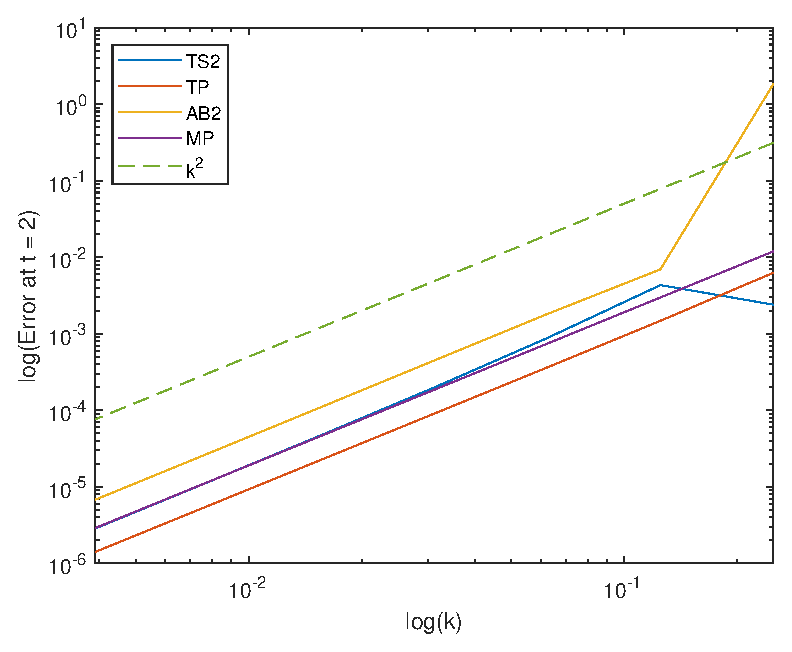
\includegraphics{p1f_plot.eps}
			\caption{Numerical errors at $t = 2$ versus time step}
			\label{fig:error_plot}
		\end{figure}
	\end{alphaparts}
	
	\question
	
\end{document}